\section{Introducción y objetivos}


\begin{frame}[c]{Motivación}

    El comportamiento de las enfermedades infecciosas es especialmente relevante en países menos desarrollados, pues sufren consecuencias más graves.
    \\~\\
    Los modelos matemáticos en epidemiología ayudan a comprender los mecanismos que intervienen en la propagación de las enfermedades y sugerir mecanismos para su control.

\end{frame}


\begin{frame}{Objetivos}

    \begin{itemize}
        \item Marcados al inicio:

        \pause
        \begin{itemize}
            \item Descripción y estudio de modelos discretos en epidemiología.
            \pause
            \item Visualización del comportamiento de los modelos.
            \pause
            \item Desarrollo de una página web.
        \end{itemize}
        
        \pause
        \item Adicionales:

        \pause
        \begin{itemize}
            \item Descripción y estudio de modelos continuos en epidemiología.
            \pause
            \item Ajuste de datos.
            \pause
            \item Ajuste de datos reales.
        \end{itemize}
    \end{itemize}

\end{frame}


%%%%%%%%%%%%%%%%%%%%%%%%%%%%%%%%%%%%%%%%%%


\section{Conceptos fundamentales}


%\begin{frame}{Conceptos fundamentales (I)}

%    \begin{block}{Epidemia}
%        Las epidemias son brotes espontáneos de una enfermedad o situaciones endémicas, en las que la enfermedad está siempre presente.
%    \end{block}  

%\end{frame}



\begin{frame}{Conceptos fundamentales (I)}

    \begin{block}{Individuos susceptibles}
        Los individuos \textbf{susceptibles}, que denotamos $S_n$, son aquellos que pueden infectarse con la enfermedad pero aún no lo han hecho en el momento $n$.
    \end{block}  

    \pause

    \begin{block}{Individuos infectados}
        Los individuos \textbf{infectados}, a los que denotamos $I_n$, son las personas infectadas en el instante $n$ por la enfermedad y pueden contagiar la enfermedad a los individuos susceptibles.
    \end{block}  

    \pause

    \begin{block}{Individuos recuperados}
        Los individuos \textbf{recuperados}, que denotamos $R_n$, son los individuos que han estado infectados y ya no contagian la enfermedad ni pueden volver a infectarse.
        Los individuos recuperados hacen referencia a los individuos inmunizados, aislados, recuperados o fallecidos.
    \end{block}  


\end{frame}


\begin{frame}{Conceptos fundamentales (II)}

    \begin{block}{Epidemia}
        Las epidemias son brotes espontáneos de una enfermedad o situaciones endémicas, en las que la enfermedad está siempre presente.
    \end{block}  

    \pause

    En todos los modelos se parte de realizan las siguientes suposiciones:

    \begin{itemize}
        \item La población se mezcla de manera homogénea, es decir, todos los individuos tienen la misma probabilidad de interactuar entre ellos y contraer la enfermedad.
        \item El total de la población es constante y lo denotaremos por $N$.
    \end{itemize}

\end{frame}


%%%%%%%%%%%%%%%%%%%%%%%%%%%%%%%%%%%%%%%%%%


\section{Modelos discretos en epidemiología}


\subsection{Modelo SI}


\begin{frame}{Modelo SI (I)}

    \begin{block}{Modelo SI}

        \begin{equation}
        \label{eqn: SI}
        \begin{aligned}
        S_{n+1}=S_n\left( 1-\frac{\alpha\Delta t}{N}I_n\right) \\
        I_{n+1}=I_n\left( 1+\frac{\alpha\Delta t}{N}S_n\right)
        \end{aligned}
        \end{equation}

        Con condiciones iniciales $S_0>0$, $I_0>0$ y $S_0+I_0=N$.
        

    \end{block}  

    %\begin{itemize}
    %    \item $S_n$: número de individuos susceptibles en el instante $t_n$.
    %    \item $I_n$: número de individuos infectados en ese instante.
    %    \item $\Delta t$: tiempo transcurrido entre dos instantes $t_{n+1}-t_n$. 
    %    \item $\alpha$ es la tasa de contacto; es decir, el número medio de individuos con los que un infectado tiene suficiente contacto para contagiarlo en un intervalo de tiempo.
    %\end{itemize}

\end{frame}

\begin{frame}{Modelo SI (II)}
 
    %\begin{proposition}
    %    Las soluciones de las ecuaciones \eqref{eqn: SI} son positivas si y solo si $\alpha\Delta t \leq 1$.
    %\end{proposition}
    
    %\pause

    \begin{lema}
        $S_n$ es monótonamente decreciente e $I_n$ es monótonamente creciente.
    \end{lema}

    \pause

    Los únicos puntos de equilibrio posibles son: $(S^*,I^*)=(0,N)$ y $(S^*,I^*)=(N,0)$.
    \\~\\
    El sistema debe converger a $(S^*,I^*)=(0,N)$.



\end{frame}

\begin{frame}{Modelo SI (III)}
    \begin{figure}
        \begin{center}
        \caption{Gráfica del modelo SI discreto, en una población total de $100$ individuos, con valores iniciales $S_0=99, I_0 = 1, \alpha = 0.1, T_0 = 0, T = 100$.}
        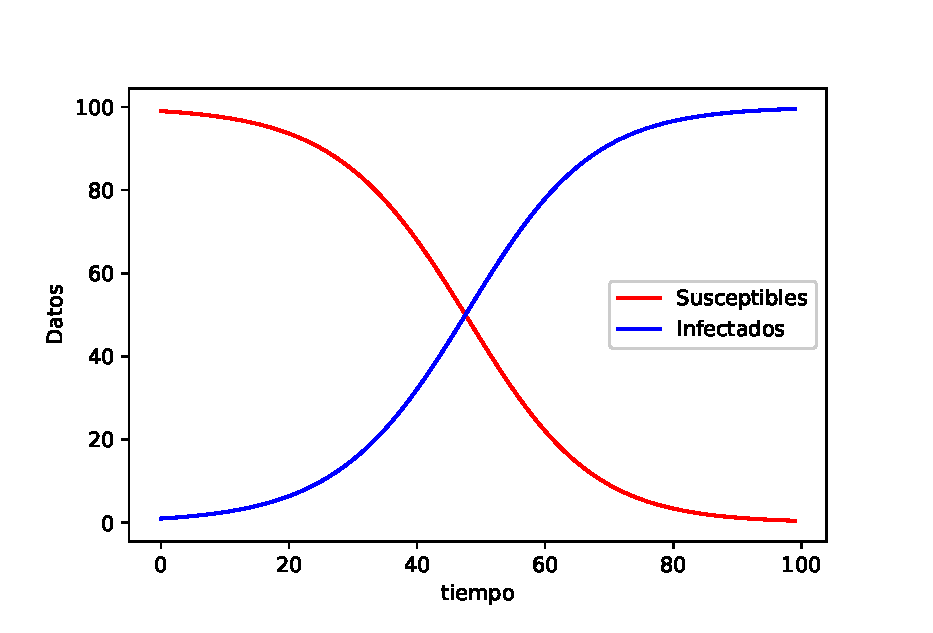
\includegraphics[scale=0.6]{graficaSI}
        \end{center}
    \end{figure}
\end{frame}


%\begin{frame}{Modelo SI (IV)}
%    \begin{figure}
%        \begin{center}
%        \caption{Gráfica del modelo SI, representando el número de infectados según el número de individuos susceptibles, en una población total de $100$ individuos, con valores iniciales $S_0=99, I_0 = 1, \alpha = 0.1, T_0 = 0, T = 100$.}
%        \label{fig: SI_IsobreS}
%        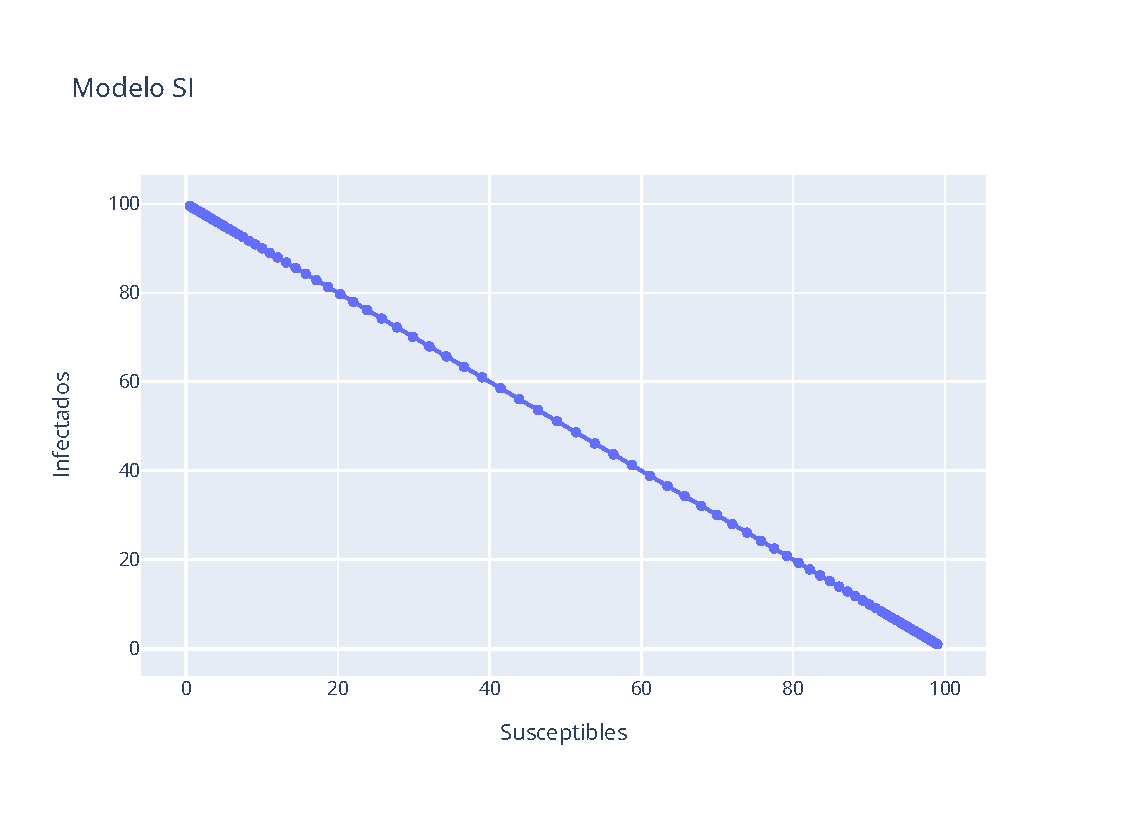
\includegraphics[scale=0.5]{SI_IsobreS}
%        \end{center}
%        \end{figure}
%\end{frame}


\subsection{Modelo SIR}


\begin{frame}{Modelo SIR (I)}

    \begin{block}{Modelo SIR}
        \begin{equation}
        \label{eqn: SIR_modelo}
        \begin{aligned}
        S_{n+1} = & S_n \left(1-\frac{\alpha\Delta t}{N} I_n \right) \\
        I_{n+1} = & I_n \left( 1-\gamma \Delta t + \frac{\alpha\Delta t}{N} S_n \right) \\
        R_{n+1} = & R_n + \gamma \Delta t I_n
        \end{aligned}
        \end{equation}
        
        Con condiciones iniciales $S_0>0$, $I_0>0$, $R_0\geq 0$, satisfaciendo $S_0+I_0+R_0=N$.
    \end{block}
\end{frame}


\begin{frame}{Modelo SIR (II)}
    %\begin{proposition}
    %    Las soluciones a este sistema discreto son positivas para cualquier valor de las condiciones iniciales si, y solo si:
    %    $$\max{\big\{\gamma\Delta t, \alpha\Delta t\big\} } \leq 1,$$
        
    %    o equivalentemente  
    %    $\min{\bigg\{ \frac{1}{\gamma}, \frac{1}{\alpha} \bigg\} } \geq \Delta t.$
        
    %    \end{proposition}

    %    \pause 

        \begin{lema}
            $S_n$ es estrictamente decreciente y $R_n$ es estrictamentre creciente.
        \end{lema}

        \pause

        \begin{definition}
            Definimos el número básico reproductivo como la constante 
            $$\mathcal{R}_{SIR}=\frac{S_0 \alpha}{N\gamma }.$$
        \end{definition}


\end{frame}

\begin{frame}{Modelo SIR (III)}
    \begin{figure}
        \begin{center}
        \caption{Gráfica del modelo SIR, en una población total de $100$ individuos, con valores iniciales $S_0=99, I_0 = 1, R_0 = 0, \alpha = 0.1, \gamma = 0.01, T_0 = 0, T = 300$.}
        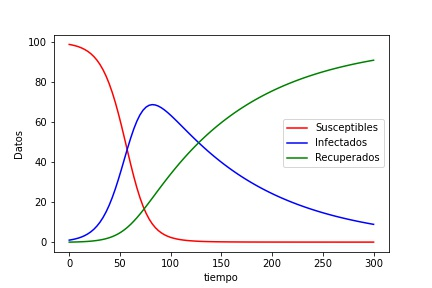
\includegraphics[scale=0.6]{graficaSIR}
        \end{center}
    \end{figure}
\end{frame}

%\begin{frame}{Modelo SIR (IV)}

%    \begin{columns}
%        \column{0.5\textwidth}
%        \begin{minipage}[c][0.4\textheight][c]{\linewidth}
%          \centering
%          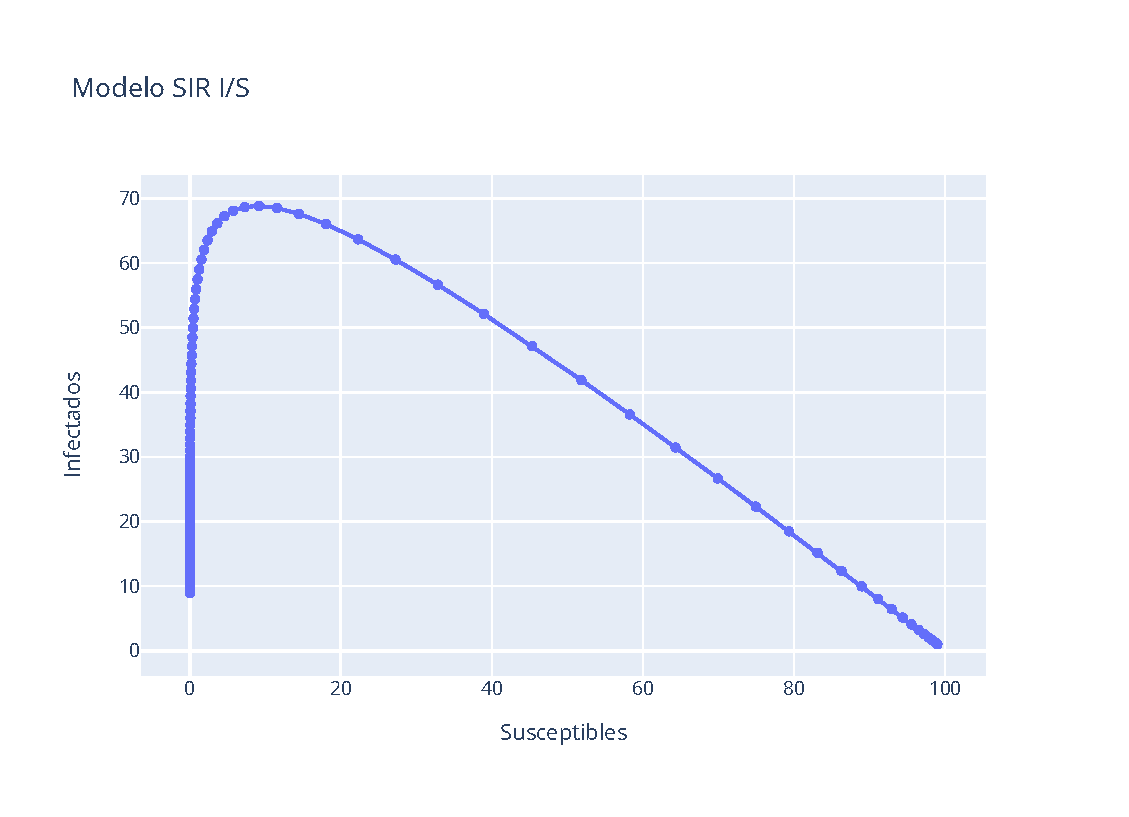
\includegraphics[width=1.2\linewidth]{SIR_IsobreS}
%        \end{minipage}
%        \begin{minipage}[c][0.4\textheight][c]{\linewidth}
%            \begin{enumerate}
%                \item Individuos infectados en función de los susceptibles.
%                \item Individuos recuperados en función de los susceptibles.
%                \item Individuos recuperados en función de los infectados.
%            \end{enumerate}
          
%        \end{minipage}
%        \column{0.5\textwidth}
%        \begin{minipage}[c][0.4\textheight][c]{\linewidth}
%            \centering
%            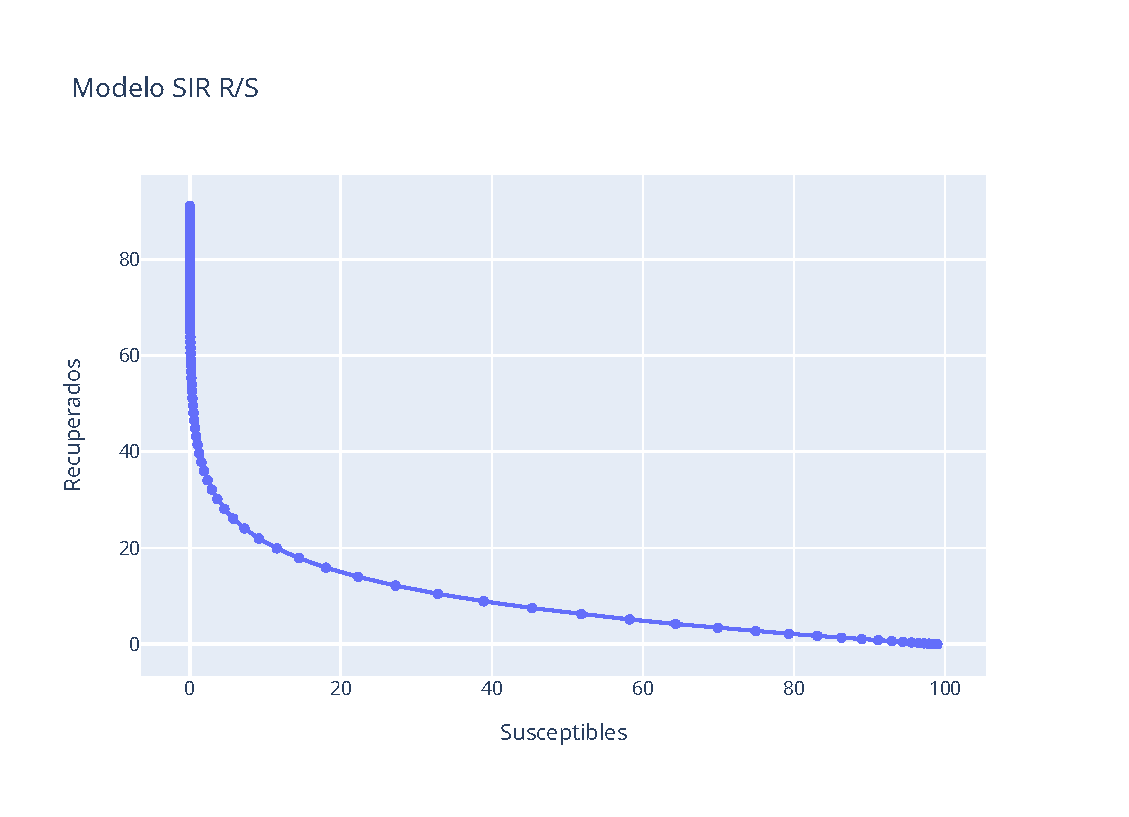
\includegraphics[width=1.2\linewidth]{SIR_RsobreS}
%        \end{minipage}
%        \begin{minipage}[c][0.4\textheight][c]{\linewidth}
%          \centering
%          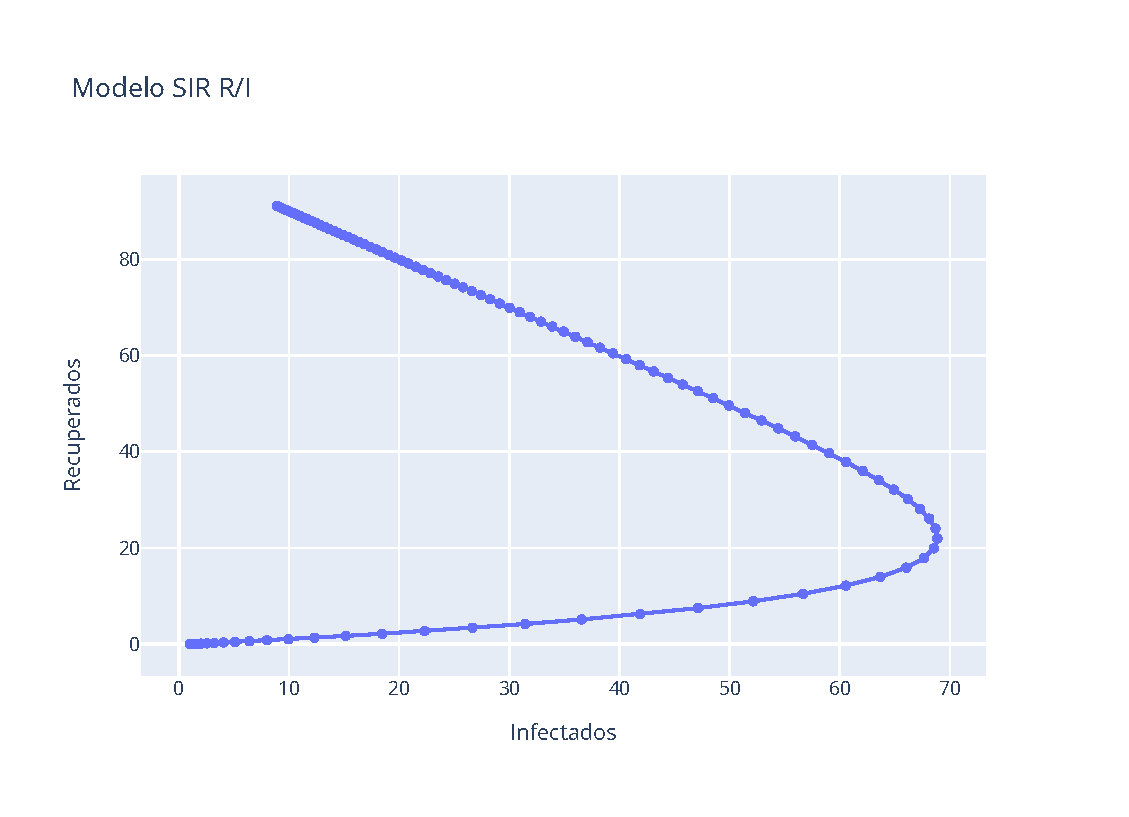
\includegraphics[width=1.2\linewidth]{SIR_RsobreI}
%        \end{minipage}
%        \end{columns}

%\end{frame}


\subsection{Modelo SIS}


\begin{frame}{Modelo SIS (I)}
    \begin{block}{Modelo SIS}
        \begin{equation}
            \label{eqn: modelo_SIS}
            \begin{aligned}
            S_{n+1} & = S_n \left(1-\frac{\alpha\Delta t}{N} I_n \right) + \gamma \Delta t I_n \\
            I_{n+1} & = I_n \left( 1-\gamma \Delta t + \frac{\alpha\Delta t}{N} S_n \right)
            \end{aligned}
            \end{equation}
            
            Con condiciones iniciales $S_0>0$, $I_0>0$ cumpliendo $S_0+I_0=N$.
    \end{block}
\end{frame}


\begin{frame}{Modelo SIS (II)}

    %\begin{proposition}
    %    Las soluciones de \eqref{eqn: modelo_SIS} siempre son positivas si, y solo si:
        
    %    $$\gamma \Delta t \leq 1 $$ y $$\alpha\Delta t< \left( 1+\sqrt{\gamma \Delta t} \right)^2$$
        
    %\end{proposition}

    \begin{lema}
        Los puntos de equilibrio de \eqref{eqn: modelo_SIS} son o bien $(S^*,I^*)=(N,0)$, o bien $(S^*,I^*)=(\frac{N\gamma}{\alpha}, N-\frac{N\gamma}{\alpha})$.
    \end{lema}

    \pause

    \begin{definition}
        El número básico reproductivo se define como 
        $$\mathcal{R}_{SIS}=\frac{\alpha}{\gamma}.$$
    \end{definition}
\end{frame}


\begin{frame}{Modelo SIS (III)}


    \begin{figure}
        \begin{center}
        \caption{Gráfica del modelo SIS, en una población total de $100$ individuos, con valores iniciales $S_0=95, I_0 = 5, \alpha = 0.1, \gamma=0.01, T_0 = 0, T = 150$.}
        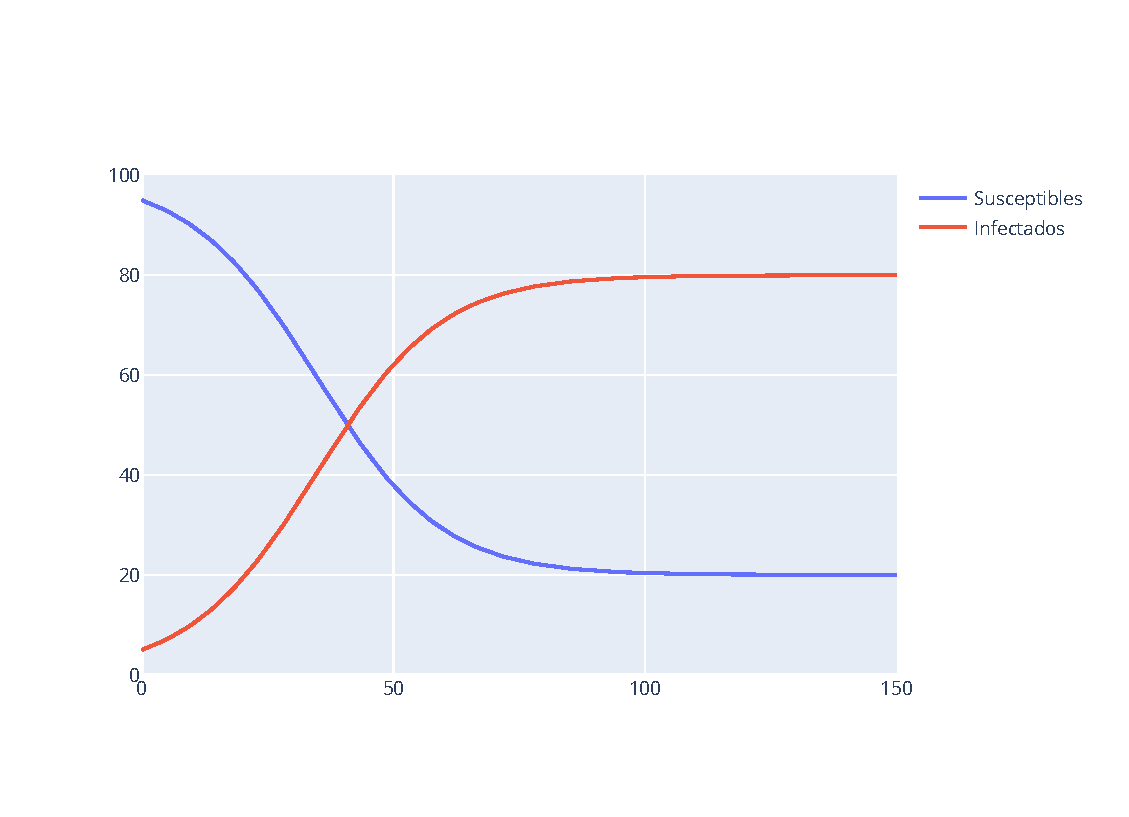
\includegraphics[scale=0.5]{SIS_modelo}
        \end{center}
    \end{figure}

\end{frame}


%%%%%%%%%%%%%%%%%%%%%%%%%%%%%%%%%%%%%%%%%%


\section{Modelos continuos en epidemiología}


\subsection{Modelo SI}


\begin{frame}{Modelo SI (I)}

    \begin{block}{Modelo SI}
        \begin{equation}
            \label{eqn:SI_continuo}
            \begin{aligned}
            S'(t) & = -\frac{\alpha}{N}SI \\
            I'(t) & = \frac{\alpha}{N}SI
            \end{aligned}
        \end{equation}
            
        Con condiciones iniciales $S(0)+I(0)=N$.
    \end{block}
    
    \pause
    De \eqref{eqn:SI_continuo} se puede ver que $I'>0$ y $S'<0$, luego ambas funciones son estrictamente monótonas
    \\~\\

    \pause
    Resolviendo el sistema de ecuaciones, vemos que las soluciones convergen a $(S^*,I^*)=(0,N)$.
\end{frame}


\begin{frame}{Modelo SI (II)}

    \begin{figure}
    \begin{center}
    \caption{Gráfica del modelo SI continuo, en una población total de $100$ individuos, con valores iniciales $S(0)=99, I(0) = 1, \alpha = 0.1,T_0 = 0, T = 100$.}
    \label{fig: SI_continuo}
    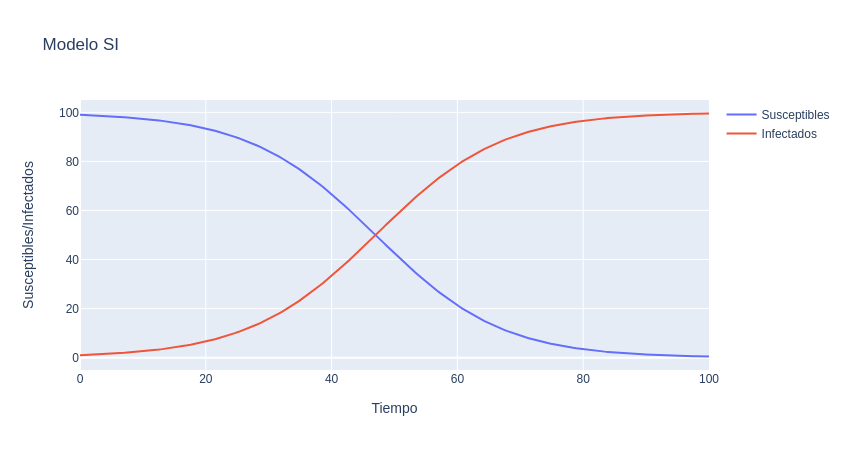
\includegraphics[scale=0.4]{SI_continuo_modelo}
    \end{center}
    \end{figure}

\end{frame}


\subsection{Modelo SIS}


\begin{frame}{Modelo SIS (I)}
    \begin{block}{Modelo SIS}
    \begin{equation}
        \label{eqn: modelo_SIS_continuo}
        \begin{aligned}
        S'(t) = & -\frac{\alpha}{N}SI+\gamma I \\
        I'(t) = & I\left( \frac{\alpha}{N}S-\gamma \right) \\
        \end{aligned}
        \end{equation}
    
        Con $S(0)+I(0)=N$. 
    \end{block}
    
    \pause
    El número básico reproductivo se define como $\mathcal{R}_{SIS}=\frac{\alpha}{\gamma}$.
        
\end{frame}


\begin{frame}{Modelo SIS (II)}
    \begin{figure}
    \begin{center}
        \caption{Gráfica del modelo SIS continuo, en una población total de $100$ individuos, con valores iniciales $S(0)=95, I(0) = 5, \alpha = 0.1, \gamma = 0.01, T_0 = 0, T = 150$.}
        \label{fig: SIS_continuo}
        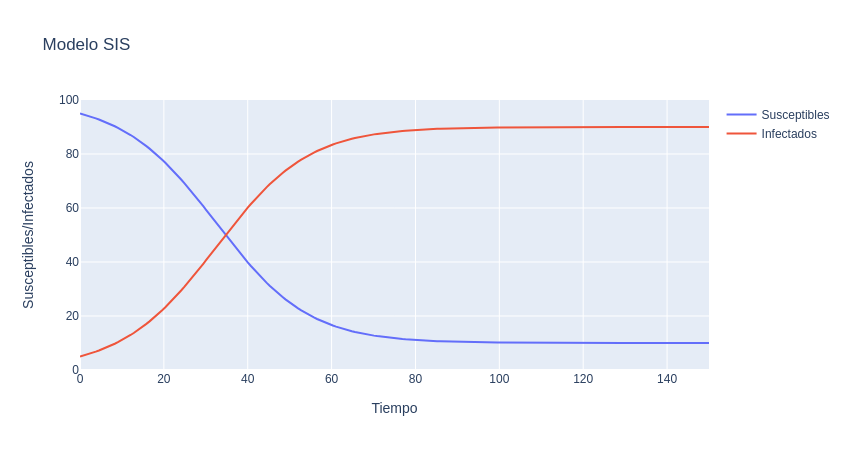
\includegraphics[scale=0.35]{SIS_continuo_modelo}
        %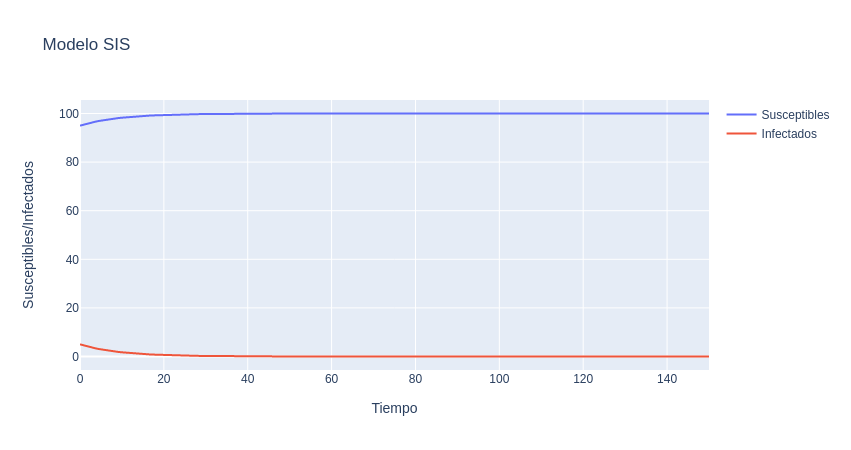
\includegraphics[scale=0.25]{SIS_continuo_modelo3}
        \end{center}
        \end{figure}

    

\end{frame}

\begin{frame}{Modelo SIS (III)}
    \begin{figure}
        \begin{center}
        \caption{Gráfica del modelo SIS continuo, en una población total de $100$ individuos, con valores iniciales $S(0)=95, I(0) = 5, \alpha = 0.1, \gamma = 0.2, T_0 = 0, T = 150$.}
        \label{fig: SIS_continuo3}
        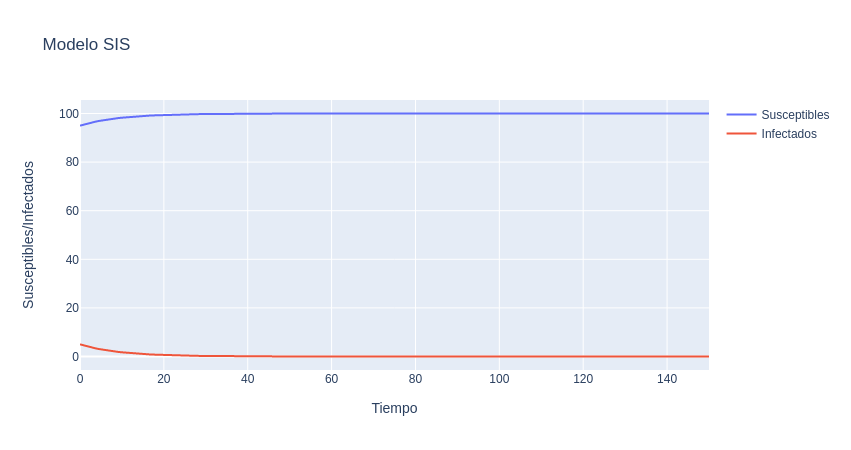
\includegraphics[scale=0.35]{SIS_continuo_modelo3}
        \end{center}
        \end{figure}

\end{frame}

\subsection{Modelo SIR}


\begin{frame}{Modelo SIR (I)}
    \begin{block}{Modelo SIR}
        \begin{equation}
            \label{eqn: modelo_SIR_continuo}
            \begin{aligned}
            S'(t) = & -\dfrac{\alpha}{N}SI \\
            I'(t) = & I\left(\dfrac{\alpha}{N}S-\gamma \right) \\
            R'(t) = & \gamma I
            \end{aligned}
            \end{equation}
            
            Con $S(0)+I(0)+R(0)=N$.
    \end{block}

    \pause
    El número básico reproductivo en este caso se define como
    $$\mathcal{R}_{SIR}=\frac{S(0)\alpha }{N\gamma }$$

\end{frame}


\begin{frame}{Modelo SIR (II)}
    \begin{figure}
        \begin{center}
        \caption{Gráfica del modelo SIR continuo, en una población total de $100$ individuos, con valores iniciales $S(0)=99, I(0) = 1, \alpha = 0.1, \gamma = 0.01, T_0 = 0, T = 300$.}
        \label{fig: SIR_continuo}
        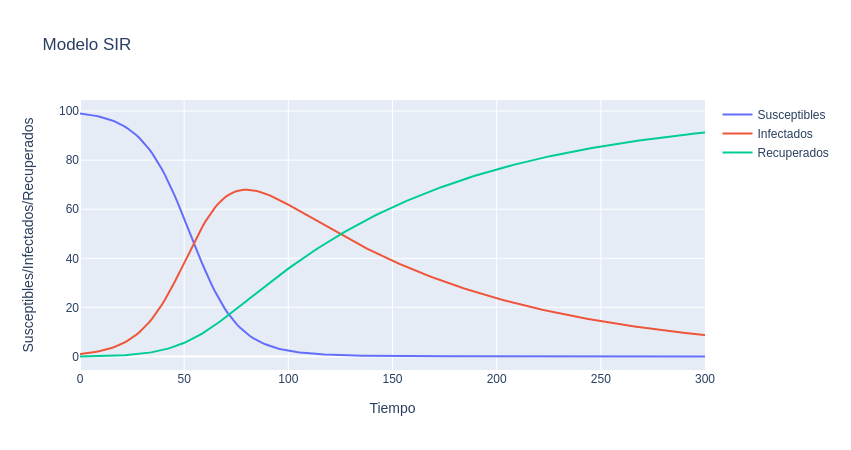
\includegraphics[scale=0.35]{SIR_continuo_modelo}
        \end{center}
        \end{figure}
\end{frame}



%%%%%%%%%%%%%%%%%%%%%%%%%%%%%%%%%%%%%%%%%%


\section{Desarrollo de la página web}


\subsection{La página web}


\begin{frame}{Herramientas}

    \begin{itemize}
        \item Gráficas interactivas $\Rightarrow$ Dash.
        \pause
        \item Framework para la web $\Rightarrow$ Flask.
        \pause
        \item Virtualización $\Rightarrow$ Docker.
        \pause
        \item Control de versiones y repositorio $\Rightarrow$ Git y Github.
        \begin{itemize}
            \item \href{https://github.com/Mapachana/TFG}{https://github.com/Mapachana/TFG}
        \end{itemize}
        \pause
        \item Ajuste de datos $\Rightarrow$ Scipy.
        \begin{itemize}
            \item Ajuste por mínimos cuadrados.
            \item Expresión de los errores como 1/MSE.
            \item Selección del mejor modelo para unos datos dados.
        \end{itemize}
    \end{itemize}

    \pause

    \href{run:/home/mapachana/2022-06-23 19-38-25.mkv}{Click for video}

\end{frame}


\subsection{Datos reales}


\begin{frame}{El Covid-19 en España}

\end{frame}


\begin{frame}{El VIH en Baleares}

\end{frame}


%%%%%%%%%%%%%%%%%%%%%%%%%%%%%%%%%%%%%%%%%%


\section{Conclusiones}


\begin{frame}{Conclusiones}

\end{frame}


%%%%%%%%%%%%%%%%%%%%%%%%%%%%%%%%%%%%%%%%%%

\begin{frame}{Referencias}
    \bibliography{../redaccion_tfg/bib/library.bib}
    \bibliographystyle{plain}
\end{frame}


\begin{frame}[c]{}
\begin{center}
\large{\textbf{Gracias por su atención.}}
\end{center}
\end{frame}
